\section{File e file system}
Un file consiste in un'astrazione offerta dal sistema operativo che lega un
blocco di byte di dimensione arbitraria ad un nome.
I nomi sono organizzati in una struttura gerarchica fatta di cartelle o
directory che permette di identificare uno specifico file attraverso una
concatenazione dei nomi di cartelle e del nome del file che ne esprime il cammino
(path) a partire da una radice nota.

Ad ogni file sono associati vincoli di sicurezza infatti il sistema operativo
garantisce che solo chi dispone delle necessarie autorizzazioni possa leggere,
scrivere o eseguire il file.

Le librerie dei linguaggi di programmazione offrono meccanismi indipendenti dal
sistema operativo per accedere al contenuto di un file.

Nel caso di Rust, l'astrazione principale è offerta da \mintinline{rust}|std::fs::File| che
modella un file aperto in lettura e/o scrittura.

Il C++, dalla versione 17, ha introdotto la libreria \mintinline{rust}{std::filesystem}.

\section{Percorsi}

Ogni sistema operativo ha regole proprie per la definizione di cosa sia un
percorso lecito per indicare un file, quali siano le radici note dei percorsi,
come combinare segmenti parziali in un percorso complessivo.

In Rust le struct \mintinline{rust}|std::path::Path| e  \mintinline{rust}|std::path::PathBuf| nascondono
tali differenze offrendo un meccanismo portabile per comporre e scomporre un cammino
e ricavare indicazioni sul file eventualmente referenziato.


\begin{itemize}
  \item \textbf{Path}, analogamente a \texttt{str}, è \verb|unsized| e accessibile in sola lettura
  \item \textbf{PathBuf}, analogamente a \texttt{String}, possiede il proprio contenuto e può
        essere modificato
\end{itemize}

Attraverso i metodi offerti da questi tipi, è possibile ricavare informazioni sulla
esistenza del file, sulla sua natura come file semplici, directory, collegamenti simbolici, ecc.,
sui metadati associati come dimensioni, data di creazione e di ultima modifica e permessi, ecc.


\section{Navigare il file system}
La funzione \mintinline{rust}|std::fs::read_dir(dir: &Path) -> Result<ReadDir>|
restituisce, se ha successo, un iteratore al contenuto della cartella dir.
Le singole voci restituite sono di tipo \texttt{std::fs::DirEntry} e descrivono gli elementi
contenuti nella cartella in termini di nome, tipo - file, cartella, collegamento simbolico -, metadati e cammino.


La funzione \mintinline{rust}|std::fs::create_dir(dir: &Path) -> Result<()>| crea
una nuova cartella.
Fallisce se non si dispone delle necessarie autorizzazioni, se la cartella
esiste già o se la cartella genitrice del cammino indicato non esiste.


La funzione \mintinline{rust}|std::fs::remove_dir(dir: &Path) -> Result<()>| rimuove una cartella,
a condizione che esista, si disponga dei necessari permessi e che sia vuota.

\section{Manipolare i file nel file system}
La funzione \mintinline{rust}|std::fs::copy(from: &Path, to: &Path) -> Result<i64>|
copia il contenuto di un file in un secondo file. Restituisce in caso di
successo il numero di byte copiati.

La funzione \mintinline{rust}|std::fs::rename(from: &Path, to: &Path) -> Result<()>| rinomina, sposta,
un file in un secondo file, sostituendo il contenuto del file destinazione con quello sorgente.
Il comportamento di questa funzione dipende dal sistema operativo.


La funzione \mintinline{rust}|std::fs::remove_file(path: &Path) -> Result<()>| elimina un file.
Se il file è in uso, la sua eliminazione può essere rimandata dal sistema operativo.


\section{Operazioni con i file}
L'accesso al blocco di byte legato ad un file è totalmente mediato dal sistema operativo.
Infatti per poter leggere o scrivere tale blocco occorre aprire il file.
Il sistema operativo offre apposite funzioni che restituiscono un riferimento
opaco al file sotto forma di handle o file descriptor, di fatto un numero
intero.

La struct \texttt{std::fs::File} di Rust offre due metodi di base per aprire un file:

\begin{itemize}
  \item[] \mintinline{rust}|open(path: P) -> Result<File> where P: AsRef<Path>| -
        apre il file in lettura, a condizione che esista
  \item[] \mintinline{rust}|create(path: P) -> Result<File> where P: AsRef<Path>| -
        tronca il file a 0 byte, se esiste, o lo crea, se non esiste ancora, dopodiché
        lo apre in scrittura
\end{itemize}


Maggiori opportunità sono offerte dalla struct \texttt{std::fs::OpenOptions}.
Essa permette di impostare come un file debba essere aperto e quali operazioni
sono consentite su di esso.


\section{Leggere e scrivere file}
Le funzioni \mintinline{rust}|std::fs::read_to_string(path: &Path)| e
\mintinline{rust}|std::fs::write(path: &Path, contents: &[u8])|
offrono un meccanismo compatto per leggere e scrivere il contenuto di un file di
moderate dimensioni.

Poiché un file può avere dimensioni molto maggiori del massimo blocco di
memoria allocabile, occorre utilizzare tali funzioni quando si è certi che il
contenuto può essere ospitato nella memoria del processo.



\begin{minted}[breaklines]{rust}
use std::fs;
let contents = fs::read_to_string(filename)
                  .expect("Something went wrong reading the file");
println!("Text is:\n{}", contents);
\end{minted}

\section{Aprire un file}

\begin{minted}[breaklines]{rust}
use std::fs::File;
use std::io::{Write, BufReader, BufRead};

let path = "lines.txt";

let mut output = File::create(path)?;
write!(output, "Rust\n<3\nFun")?;

let input = File::open(path)?;
let buffered = BufReader::new(input);

for line in buffered.lines() {
  println!("{}", line?);
}
\end{minted}

\section{I tratti relativi a I/O}


\begin{center}
  \begin{minipage}{0.65\linewidth}
    Rust gestisce le operazioni di I/O attraverso l'utilizzo di alcuni
    tratti che implementano i metodi di base per le attività di lettura e
    scrittura. L'utilizzo di tratti favorisce la scrittura di codice generico,
    indipendente dal tipo specifico su cui viene eseguito.

    I tratti principali offerti da Rust sono: \verb|Read|, \verb|BufRead|, \verb|Write| e \verb|Seek|.
    Tutti e quattro i tratti possono essere importati in maniera concisa attraverso il costrutto
    \texttt{use std::io::prelude::*}.


    In caso di errore durante le operazioni di I/O viene restituita una delle varianti
    disponibili nell'enum \texttt{std::io::ErrorKind}. La variante \texttt{std::io::ErrorKind::Interrupted}
    indica un errore non fatale, che generalmente può essere gestito
    riprovando l'operazione.

  \end{minipage}%
  \hfill
  \begin{minipage}{0.3\linewidth}
    \centering
    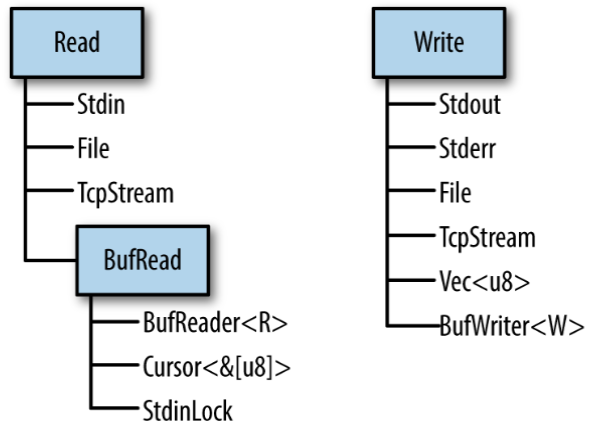
\includegraphics[width=\linewidth]{content/API_Programming/images/2026-04-03-11-50-47.png}
  \end{minipage}
\end{center}

\subsection{std::io::Read}
Tratto che indica la capacità di leggere un flusso di byte.
\verb|File|, \verb|Stdin| e \verb|TcpStream| sono alcuni dei tipi che implementano questo tratto.


Per implementare il tratto \verb|Read| è sufficiente fornire l'implementazione
del metodo \\ \mintinline{rust}|read(buf: &mut [u8]) -> Result<usize>|.

Rust genererà tutti gli altri metodi sulla base dell'implementazione di \texttt{read(buf: \&mut [u8])}
fornita dal programmatore.

In caso di successo, il metodo \texttt{read(buf: \&mut [u8])} deve ritornare \texttt{Ok(n)}.


\begin{itemize}
  \item L'implementazione deve garantire che \textit{n} sia compreso tra 0 e \texttt{buf.len()}
  \item Il valore \textit{Ok(0)} può indicare che il flusso è terminato oppure
        che il buffer passato ha lunghezza 0.
\end{itemize}

Ogni chiamata al metodo \texttt{read(buf: \&mut [u8])}  può causare l'invocazione
di una chiamata di sistema, con il conseguente costo legato al cambio di contesto.

\begin{minted}[breaklines]{rust}
use std::io::{self, Read};

struct MyReader {
    data: Vec<u8>,
    pos: usize,
}

impl Read for MyReader {
    fn read(&mut self, buf: &mut [u8]) -> io::Result<usize> {
        let remaining = &self.data[self.pos..];
        let n = remaining.len().min(buf.len());
        buf[..n].copy_from_slice(&remaining[..n]);
        self.pos += n;
        Ok(n)
    }
}

fn main() {
    let mut reader = MyReader { data: b"ciao".to_vec(), pos: 0 };
    let mut out = String::new();
    reader.read_to_string(&mut out).unwrap();
    println!("{out}"); // "ciao"
}
\end{minted}


\subsection{Metodi del tratto Read}
L'implementazione del tratto \verb|Read| mette a disposizione diversi metodi per gestire
le operazioni più comuni di I/O

\begin{description}
  \item[\texttt{read\_to\_end(buf: \&mut Vec<u8>) -> Result<usize>}] - continua a leggere
        fino all'EOF: si limita a richiamare il metodo \texttt{read()} fino a
        quando quest'ultimo non ritorna un valore \texttt{Ok(0)} o un errore fatale.
  \item[\texttt{read\_to\_string(buf: \&mut String) -> Result<usize>}] - continua a
        leggere fino all'EOF e riceve come parametro una \texttt{\&mut String}.
  \item[\texttt{read\_exact(buf: \&mut [u8]) -> Result<()>}] - prova a leggere l'esatto
        numero di byte necessario a riempire completamente \textit{buf}; se non
        riesce ritorna \verb|ErrorKind::UnexpectedEof|.
  \item[\texttt{bytes() -> Bytes<Self>}] - ritorna un iteratore sui byte, gli
        elementi dell'iteratore sono dei \texttt{Result<u8, io::Error>}
  \item[\texttt{chain<R: Read>(next: R) -> Chain<Self, R>}] - permette di concatenare due reader
  \item[\texttt{take(limit: u64) -> Take<Self>}]  - limita il numero di byte che possono essere letti da un reader
\end{description}


\section{std::io::BufRead}

Il tratto \verb|BufRead|  offre una serie di metodi che permettono di migliorare le
prestazioni dell'I/O appoggiandosi ad un buffer in memoria.

\begin{itemize}
  \item Ogni chiamata a \texttt{read()} può dare origine ad una system call,
        l'utilizzo di un buffer permette di effettuare meno chiamate
  \item Risulta particolarmente efficace se si eseguono molte letture di piccole dimensioni
  \item  Non è utile quando si legge da elementi già presenti in memoria
\end{itemize}

L'implementazione del tratto richiede i metodi \texttt{fill\_buf()}  e \texttt{consume(amt: usize)}.
I due metodi devono sempre essere utilizzati insieme: \texttt{fill\_buf()} si
limita a ritornare il contenuto del buffer in memoria, successivamente è
necessario chiamare il metodo \texttt{consume(\dots)} per garantire che i byte non siano ritornati nuovamente.


Offre i metodi \texttt{read\_line(\&mut self, buf: \&mut String)} e \texttt{lines(self)}
per accedere al contenuto testuale di un file.

\begin{minted}[breaklines]{rust}
use std::io;
use std::io::prelude::*;

let stdin = io::stdin(); // stdin non implementa il tratto BufRead
let mut handle = stdin.lock(); // lock permette di ottenere uno StdinLock che implementa BufRead

let buffer = handle.fill_buf().unwrap();
println!("{:?}", buffer);

let length = buffer.len();
handle.consume(length); // garantisce che i byte letti non vengano
\end{minted}


\section{std::io::Write}
Tratto che indica la capacità di scrivere un flusso di dati. Questo tratto è
implementato, tra gli altri, dalle struct \texttt{File}, \texttt{Stdout} e \texttt{TcpStream}.

Il tratto \verb|Write| richiede l'implementazione dei metodi \textit{write} e \textit{flush}.

\begin{itemize}
  \item[] \mintinline{rust}|write(buf: &[u8]) -> Result<usize>| - prova a
        scrivere l'intero contenuto del buffer ricevuto come argomento e ritorna il
        numero di byte scritti
  \item[] \mintinline{rust}|flush() -> Result<()>| - finalizza l'output
        garantendo che tutti gli eventuali buffer transitori siano correttamente
        svuotati
\end{itemize}


\section{std::io::Seek}
Tratto che permette di ri-posizionare il cursore di lettura/scrittura in un flusso di byte.
Quando il flusso attinge ad un dato di dimensione nota, è possibile posizionare
il cursore in modo relativo rispetto all'inizio del flusso, \texttt{SeekFrom::Start(n: u64)},
alla sua fine \texttt{SeekFrom::End(n: i64)} o alla posizione corrente \texttt{SeekFrom::Current(n: i64)}.

Il tratto offre i seguenti metodi:

\begin{itemize}
  \item \texttt{fn seek(\&mut self, pos: SeekFrom) -> Result<u64>}: posiziona il cursore alla posizione
        (in byte) indicata dal parametro pos e ritorna la nuova posizione del cursore
  \item \texttt{fn rewind(\&mut self) -> Result<()>}: posiziona il
        cursore all'inizio del flusso
  \item \texttt{fn stream\_position(\&mut self) -> Result<u64>}: restituisce la
        posizione corrente del cursore rispetto all'inizio del flusso
\end{itemize}


\paragraph{Esempio: lettura di un file contenente dati binari}
\begin{minted}[breaklines]{rust}
use std::fs::File;
use std::io::Read;
fn main() -> std::io::Result<()> {
  // "/dev/urandom": sorgente di byte casuali provenienti da una sorgente sicura
  let mut f = File::open("/dev/urandom")?;

  loop {
    let mut buff = [0;4];                               // buffer in cui depositare i byte
    let r = f.read_exact(&mut buff);                    // lettura del file
    if r.is_err() { return r; }
    if buff.iter().any(|b| *b==0) { return Ok(()); }    // se trovo un byte nullo, termino
    let i = i32::from_be_bytes(buff);                   // conversione del buffer in i32
    println!("{:x}",i);                                 // uso il valore letto
  }
}
\end{minted}


\section{Lettura e scrittura di contenuti strutturati}
Sebbene sia possibile operare a livello di singoli byte/caratteri e ricostruire
un dato strutturato a partire dai suoi componenti elementari, spesso è poco
conveniente farlo.

Rust mette a disposizione il framework \texttt{Serde} il cui scopo è generare
implementazioni efficienti di funzioni di serializzazione e deserializzazione di
strutture dati arbitrarie verso formati standard quali \verb|JSON|, \verb|YAML|, \verb|CSV|,
\verb|BSON|, \verb|Avro|, \verb|XML|  e tanti altri.


Tale framework definisce i tratti \texttt{serde::Serialize} e \texttt{serde::Deserialize}
che possono essere implementati dai tipi definiti all'interno di un programma.

\texttt{Serde} offre un'implementazione predefinita per la serializzazione dei tipi
elementari e di alcuni tipi della libreria standard.

\begin{itemize}
  \item[] \texttt{String}, \texttt{\&str}, \texttt{Vec<T>}, \texttt{HashMap<K, V>}, etc.
  \item[] Supporta inoltre la macro \texttt{\#[derive(Serialize, Deserialize)]}
        per generare, in fase di compilazione, l'implementazione dei tratti
        corrispondenti, a condizione che la struttura dati cui tale macro è applicata
        non contenga elementi ``patologici''
\end{itemize}


\subsection{Uso del framework Serde}
Si inseriscono, nel file Cargo.toml, le dipendenze

\begin{itemize}
  \item \verb|serde = { version = "1.0", features = ["derive"] }|
  \item \verb|serde_json = "1.0"|
\end{itemize}


La seconda indica il tipo di formato da generare/leggere.
In alternativa, è possibile indicare un altro sotto-progetto compatibile come
\verb|csv  = "1.3"| o \verb|bson = "2.9"|.

Si decora la struttura dati da leggere con la macro \texttt{\#[derive(\dots)]}
\begin{minted}[breaklines]{rust}
#[derive(Serialize, Deserialize, Debug)]
struct Data {
  name: String,
  data: Vec<u8>,
  attributes: HashMap<String, String>,
}
\end{minted}

\begin{center}
  \begin{minipage}{0.5\linewidth}
    \begin{minted}[breaklines]{rust}
fn save(data: &Data, path: &str) -> Result<()> {
  let mut f = File::options()
                    .write(true)
                    .create(true)
                    .truncate(true)
                    .open(path)?;

  f.write_all(
      serde_json::to_string(data)?
      .as_bytes()
    )?;
  Ok(())
}
\end{minted}
  \end{minipage}%
  \hfill
  \begin{minipage}{0.45\linewidth}
    \begin{minted}[breaklines]{rust}
fn load(path: &str) -> Result<Data> {
  let mut f = File::open(path)?;
  
  let mut s = String::new();
  
  f.read_to_string(&mut s)?;
  
  return Ok(serde_json::from_str(&s)?);
}
\end{minted}
  \end{minipage}
\end{center}



